\documentclass[conference]{IEEEtran}
\IEEEoverridecommandlockouts

\usepackage{cite}
\usepackage{amsmath,amssymb,amsfonts}
\usepackage{algorithm}
\usepackage{algorithmic}
\usepackage{graphicx}
\usepackage{textcomp}
\usepackage{xcolor}
\usepackage{booktabs}
\usepackage{url}
\usepackage{tikz}
\usetikzlibrary{arrows.meta, positioning, shapes.geometric, fit}

\def\BibTeX{{\rm B\kern-.05em{\sc i\kern-.025em b}\kern-.08em
    T\kern-.1667em\lower.7ex\hbox{E}\kern-.125emX}}

\begin{document}

\title{Hybrid TPA-Agent: A Decoupled Four-Layer Architecture with Deterministic Geometry, Walk-Forward ML, CoT Reasoning, and Veto Risk Governance for Short-Term Trading}

\author{
\IEEEauthorblockN{Ping-He Yeh}
\IEEEauthorblockA{\textit{Graduate Institute of Biomedical Engineering} \\
\textit{National Chung Hsing University} \\
Taichung, Taiwan \\
pinghe.yeh@gmail.com}
}

\maketitle

\begin{abstract}
Short-term traders must synthesize price structure, volatility regimes, transaction friction, and downside risk under strict time constraints. Empirical studies demonstrate that the vast majority of active individual day traders lose money over sustained horizons, highlighting the need for objective, risk-first decision support rather than unconstrained signal generation. Existing automated paradigms suffer from complementary failure modes: classical technical indicators lag non-stationary price structure, standalone machine learning classifiers are susceptible to look-ahead bias and regime overfitting, and monolithic Large Language Model (LLM) trading agents exhibit numerical and spatial hallucinations when interpreting raw candlestick charts. To address these gaps, we present \textbf{Hybrid TPA-Agent}, a decoupled four-layer, eight-module trading intelligence architecture governed by specification-driven development (OpenSpec). Layer~1 captures trader risk budgets and causal OHLCV indicators including Average True Range (ATR) and volume Z-scores. Layer~2 computes 100\% deterministic swing extrema, supply/demand zones, and Support/Resistance (S/R) flips, passing five leak-free geometric and price-action features to an XGBoost conditional win-rate filter ($W \ge 0.55$). Layer~3 pairs a curated Price Action Knowledge Base with a Chain-of-Thought (CoT) reasoning agent that is strictly prohibited from altering numerical coordinates. Layer~4 enforces an independent risk management engine holding absolute veto authority (\texttt{NO\_TRADE}) via mandatory risk-reward ($RR \ge 2.0$), positive mathematical expectation ($E > 0$), dynamic $1.0 \times \text{ATR}$ stop-loss placement, and multi-tier circuit breakers. We verify the implemented pipeline via deterministic unit/integration tests ($5/5$ passing), present an interactive Human-in-the-Loop (HITL) Streamlit audit interface, and formalize an anti-leakage walk-forward evaluation protocol across six baselines and transaction-cost sweeps.
\end{abstract}

\begin{IEEEkeywords}
Financial AI Agents, Algorithmic Trading, Risk Governance, Price Action Geometry, Chain-of-Thought Reasoning, Walk-Forward Validation, OpenSpec.
\end{IEEEkeywords}

\section{Introduction}
Retail and short-term discretionary traders operate in high-noise, non-stationary markets where cognitive overload and emotional biases severely degrade execution quality. A landmark empirical investigation of 1,551 persistent Brazilian equity-index futures day traders active for more than 300 days found that \textbf{97\% suffered net financial losses}, only 1.1\% earned more than the Brazilian minimum wage, and trading experience did not monotonically translate into profitability~\cite{chague2019day}. Complementing these findings, regulatory disclosures from the Financial Industry Regulatory Authority (FINRA Rule~2270 and Regulatory Notice~24-13) emphasize that high-frequency transaction friction, thin liquidity, leverage amplification, and API/connectivity disruptions routinely cause severe capital depletion even among market participants with substantial domain knowledge~\cite{finra2270,finra2413}. For example, FINRA illustrates that paying \$16 per round-trip in commissions and spreads across 29 daily trades requires approximately \$111,360 in annualized gross profit merely to break even~\cite{finra2270}.

Despite rapid advances in quantitative modeling and generative artificial intelligence, existing automated trading approaches exhibit three structural limitations:
\begin{enumerate}
    \item \textbf{Lagging Indicators and Pure Machine Learning:} Moving-average crossovers and oscillator rules suffer from inherent lag and generate excessive whipsaw trades in range-bound regimes, while standalone machine learning classifiers trained without structural geometry struggle under non-stationary market shifts.
    \item \textbf{Spatial and Numerical Hallucinations in Pure LLM Agents:} While Large Language Models (LLMs) excel at semantic synthesis and Chain-of-Thought (CoT) narrative generation~\cite{wei2022chainofthought}, recent research warns that LLM financial hallucinations propagate through tool-calling pipelines into erroneous position sizes, misplaced stop-losses, and cascading losses~\cite{xia2026agentic}.
    \item \textbf{Static Support/Resistance Tools:} Heuristic tools such as pivot points or kernel density estimates plot static horizontal levels without estimating conditional breakout/rebound probabilities or enforcing mathematical expectation gates.
\end{enumerate}

To overcome these weaknesses, we propose \textbf{Hybrid TPA-Agent}, founded on a strict separation-of-concerns principle: \emph{deterministic algorithms handle exact spatial geometry, machine learning estimates conditional signal quality, the LLM performs contextual narrative auditing, and an independent risk engine retains absolute veto power.} The system does not claim automated guaranteed profits; instead, it enforces statistical expectancy ($E > 0$) and Human-in-the-Loop (HITL) auditability while actively suppressing low-quality exposures via deterministic \texttt{NO\_TRADE} decisions.

The primary contributions of this paper are summarized as follows:
\begin{itemize}
    \item \textbf{Decoupled Four-Layer, Eight-Module Architecture:} We design and implement a modular trading decision pipeline isolating data ingestion (Layer~1), deterministic supply/demand geometry and XGBoost filtering (Layer~2), knowledge-grounded CoT reasoning (Layer~3), and veto-enabled risk governance with HITL audit cards (Layer~4).
    \item \textbf{Zero-Arithmetic LLM Boundary:} Unlike end-to-end LLM traders, Layer~3 receives structured JSON coordinates from Layer~2 and is explicitly constrained from performing arithmetic or modifying entry, stop-loss, or target levels.
    \item \textbf{Deterministic Veto and Circuit-Breaker Governance:} Layer~4 enforces $RR \ge 2.0$, $E = W \cdot RR - (1 - W) > 0$, dynamic $1.0 \times \text{ATR}_{14}$ structural buffers, consecutive-loss locks, and data-latency kill switches.
    \item \textbf{OpenSpec Specification-Driven Governance:} All behavioral invariants and future extensions are codified under the OpenSpec SDD framework (\texttt{openspec/}) alongside an open-source Python/Streamlit prototype and reproducible verification suite.
\end{itemize}

\section{Related Work and Empirical Motivation}
\subsection{Retail Trading Risks and Friction Asymmetry}
Chagu{\^e} et al.~\cite{chague2019day} provide large-scale evidence that retail short-term trading is characterized by negative net expectancy once commissions, spreads, and behavioral overtrading are accounted for. FINRA Rule~2270~\cite{finra2270} and Regulatory Notice~24-13~\cite{finra2413} corroborate that execution discipline, hard stop-loss enforcement, leverage caps, and operational resilience against API outages are as decisive as signal accuracy itself. These regulatory and empirical realities directly motivate our design of Layer~4 as an unbypassable veto gate rather than an advisory post-processor.

\subsection{LLM Trading Agents and Long-Horizon Critique}
Recent financial agent literature highlights two major pitfalls when deploying LLMs in live markets. First, Xia et al.~\cite{xia2026agentic} analyze perception-memory-reasoning-execution pipelines and demonstrate that numerical or spatial hallucinations in LLM outputs can cascade through tool invocations into catastrophic order sizing. Second, Li et al.~\cite{li2026finsaber} introduce the FINSABER evaluation framework spanning more than 100 assets over 2004--2024 and show that many LLM-based timing strategies claiming superior performance degrade sharply once evaluated across broad asset universes, long horizons, and realistic transaction costs.

\subsection{Gradient Boosting, Volatility Scaling, and CoT Reasoning}
Gradient boosted decision trees such as XGBoost~\cite{chen2016xgboost} remain highly effective for tabular financial features when paired with strict chronological validation. Meanwhile, Wilder's Average True Range (ATR)~\cite{wilder1978new} provides a standard volatility-normalized ruler for adaptive stop placement across changing market regimes. Finally, Chain-of-Thought (CoT) prompting~\cite{wei2022chainofthought} improves reasoning transparency when anchored to structured inputs and curated domain knowledge. Hybrid TPA-Agent synthesizes these three pillars while preventing any single component from exceeding its domain of reliability.

\section{System Architecture: Decoupled Four-Layer Design}
Figure~\ref{fig:architecture} illustrates the end-to-end data flow across the four decoupled layers and eight modules of Hybrid TPA-Agent.

\begin{figure*}[t]
\centering
\resizebox{\textwidth}{!}{%
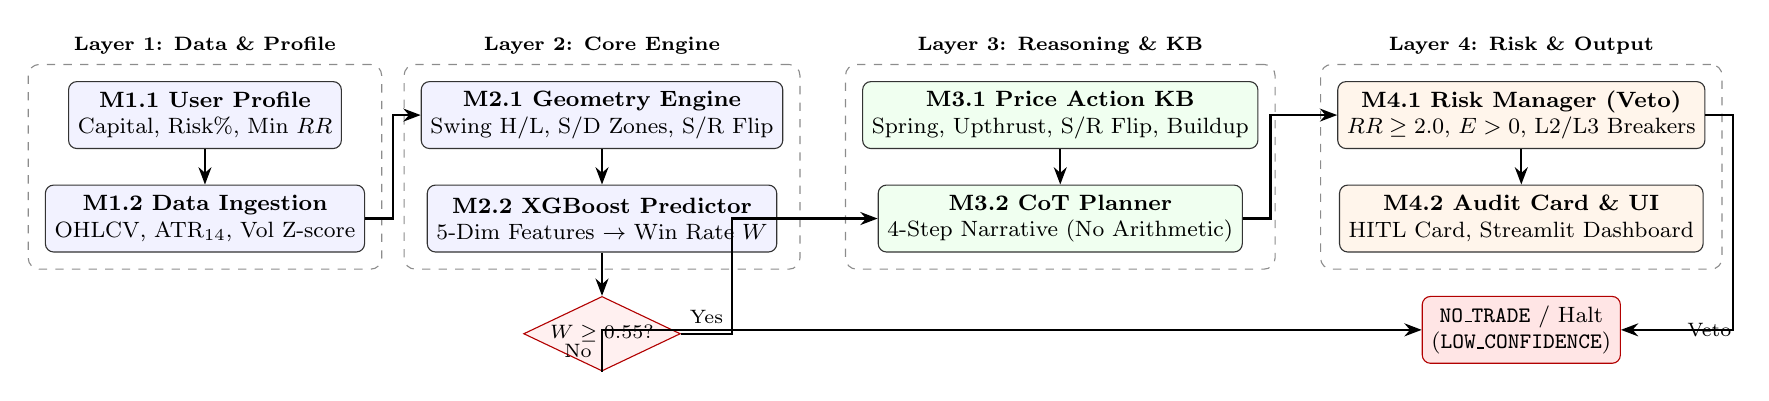
\begin{tikzpicture}[
    node distance=0.6cm and 0.9cm,
    box/.style={rectangle, draw=black!80, rounded corners=3pt, minimum width=3.3cm, minimum height=0.85cm, align=center, font=\footnotesize, fill=blue!5},
    gate/.style={diamond, aspect=2.1, draw=red!70!black, fill=red!6, align=center, font=\scriptsize, inner sep=1pt},
    veto/.style={rectangle, draw=red!70!black, rounded corners=3pt, fill=red!10, align=center, font=\footnotesize, minimum width=2.4cm, minimum height=0.7cm},
    layerbox/.style={rectangle, draw=black!45, dashed, rounded corners=4pt, inner sep=6pt},
    arrow/.style={-{Stealth[length=2.2mm]}, thick}
]
% Layer 1
\node[box] (m11) {\textbf{M1.1 User Profile}\\Capital, Risk\%, Min $RR$};
\node[box, below=0.45cm of m11] (m12) {\textbf{M1.2 Data Ingestion}\\OHLCV, $\text{ATR}_{14}$, Vol Z-score};

% Layer 2
\node[box, right=1.0cm of m11] (m21) {\textbf{M2.1 Geometry Engine}\\Swing H/L, S/D Zones, S/R Flip};
\node[box, below=0.45cm of m21] (m22) {\textbf{M2.2 XGBoost Predictor}\\5-Dim Features $\rightarrow$ Win Rate $W$};

% Gate W >= 0.55
\node[gate, below=0.55cm of m22] (gw) {$W \ge 0.55$?};

% Layer 3
\node[box, right=1.0cm of m21, fill=green!6] (m31) {\textbf{M3.1 Price Action KB}\\Spring, Upthrust, S/R Flip, Buildup};
\node[box, below=0.45cm of m31, fill=green!6] (m32) {\textbf{M3.2 CoT Planner}\\4-Step Narrative (No Arithmetic)};

% Layer 4
\node[box, right=1.0cm of m31, fill=orange!8] (m41) {\textbf{M4.1 Risk Manager (Veto)}\\$RR \ge 2.0$, $E>0$, L2/L3 Breakers};
\node[box, below=0.45cm of m41, fill=orange!8] (m42) {\textbf{M4.2 Audit Card \& UI}\\HITL Card, Streamlit Dashboard};

% Veto output
\node[veto, below=0.55cm of m42] (notrade) {\texttt{NO\_TRADE} / Halt\\(\texttt{LOW\_CONFIDENCE})};

% Layer dashed boxes
\node[layerbox, fit=(m11)(m12), label={[font=\scriptsize\bfseries]above:Layer 1: Data \& Profile}] {};
\node[layerbox, fit=(m21)(m22), label={[font=\scriptsize\bfseries]above:Layer 2: Core Engine}] {};
\node[layerbox, fit=(m31)(m32), label={[font=\scriptsize\bfseries]above:Layer 3: Reasoning \& KB}] {};
\node[layerbox, fit=(m41)(m42), label={[font=\scriptsize\bfseries]above:Layer 4: Risk \& Output}] {};

% Arrows
\draw[arrow] (m11) -- (m12);
\draw[arrow] (m12.east) -- ++(0.35,0) |- (m21.west);
\draw[arrow] (m21) -- (m22);
\draw[arrow] (m22) -- (gw);
\draw[arrow] (gw.east) -- node[above, font=\scriptsize]{Yes} ++(0.65,0) |- (m32.west);
\draw[arrow] (gw.south) |- node[near start, left, font=\scriptsize]{No} (notrade.west);
\draw[arrow] (m31) -- (m32);
\draw[arrow] (m32.east) -- ++(0.35,0) |- (m41.west);
\draw[arrow] (m41) -- (m42);
\draw[arrow] (m41.east) -- ++(0.35,0) |- node[near end, right, font=\scriptsize]{Veto} (notrade.east);
\end{tikzpicture}%
}
\caption{Decoupled four-layer, eight-module architecture of Hybrid TPA-Agent. Deterministic geometry and XGBoost probability estimation precede CoT narrative reasoning, while Layer~4 retains final veto authority.}
\label{fig:architecture}
\end{figure*}

\subsection{Layer 1: Input and Data Ingestion}
\begin{itemize}
    \item \textbf{Module 1.1 (User Preferences):} Encapsulated in \texttt{UserProfile}, this module specifies account capital $C$ (default \$10,000), per-trade risk budget $\rho_{\text{risk}}$ (default $1.0\%$), daily drawdown cap $\rho_{\text{daily}} = 3.0\%$, minimum risk-reward threshold $RR_{\min} = 2.0$, minimum conditional win rate $W_{\min} = 0.55$, and maximum leverage ($5.0\times$). The hard per-trade loss budget is $B_{\max} = C \cdot \rho_{\text{risk}}$.
    \item \textbf{Module 1.2 (Data Ingestion Engine):} Produces strictly time-ordered OHLCV series enriched causally with 14-period Average True Range ($\text{ATR}_{14}$)~\cite{wilder1978new} and 20-period rolling volume Z-scores ($\text{Vol}_{z}$), eliminating look-ahead bias during feature construction.
\end{itemize}

\subsection{Layer 2: Core Analysis Engine}
\begin{itemize}
    \item \textbf{Module 2.1 (Supply \& Demand Arithmetic Engine):} Executes purely deterministic Python geometry (\texttt{detect\_swing\_points} and \texttt{calculate\_supply\_demand\_zones}) to compute swing highs, swing lows, rectangular demand/supply zone bounds, and Support/Resistance (S/R) flip flags.
    \item \textbf{Module 2.2 (Win-Rate Prediction Engine):} \texttt{XGBWinRatePredictor} extracts a five-dimensional feature vector from the latest bar and active zone, outputting a conditional win probability $W$. Candidates with $W < W_{\min}$ ($0.55$) are filtered before entering LLM reasoning.
\end{itemize}

\subsection{Layer 3: Reasoning and Domain Knowledge}
\begin{itemize}
    \item \textbf{Module 3.1 (Price Action Knowledge Base):} Curates four structured price-action patterns (\texttt{SR\_FLIP}, \texttt{SPRING\_FALSE\_BREAKOUT}, \texttt{UPTHRUST\_FALSE\_BREAKOUT}, and \texttt{PRE\_BREAKOUT\_BUILDUP}) with explicit triggering conditions and invalidation criteria.
    \item \textbf{Module 3.2 (CoT Planning Agent):} Serializes Layer~2 geometry and probability metadata alongside the knowledge base into a structured four-step CoT prompt. The agent is explicitly instructed never to perform numerical arithmetic or mutate coordinate bounds, producing human-auditable market regime, liquidity narrative, and structural invalidation summaries.
\end{itemize}

\subsection{Layer 4: Risk Management and Output}
\begin{itemize}
    \item \textbf{Module 4.1 (Decision \& Risk Control Engine):} \texttt{RiskManager} acts as the system's supreme veto authority, executing operational circuit breakers, ATR-buffered stop-loss computation, $RR$ and $E > 0$ checks, and exact risk-budget position sizing.
    \item \textbf{Module 4.2 (Audit Interface):} \texttt{ReportGenerator} assembles a structured Audit Card containing decision status (\texttt{APPROVED} or \texttt{NO\_TRADE}), exact price levels, position size, CoT evidence, and a mandatory \texttt{human\_confirmation\_required = True} flag rendered in a Plotly/Streamlit HITL dashboard.
\end{itemize}

\section{Mathematical Formulation and Risk Governance}
\subsection{Deterministic Price Geometry}
Given a window half-width $k$ (default $k = 5$ in \texttt{app.py}, $k = 4$ in unit tests), bar $t \in [k, T - k - 1]$ is classified as a \textit{Swing High} or \textit{Swing Low} via:
\begin{align}
\text{SwingHigh}_t &\iff H_t = \max_{j \in [t-k,\, t+k]} H_j, \\
\text{SwingLow}_t  &\iff L_t = \min_{j \in [t-k,\, t+k]} L_j,
\end{align}
where $H_t$ and $L_t$ denote high and low prices. Each swing point induces a bounded Supply/Demand zone $[Z_{\text{low}}, Z_{\text{high}}]$:
\begin{equation}
\text{Demand:} \quad Z_{\text{low}} = L_t, \quad Z_{\text{high}} = \min(O_t, C_t),
\end{equation}
\begin{equation}
\text{Supply:} \quad Z_{\text{low}} = \max(O_t, C_t), \quad Z_{\text{high}} = H_t.
\end{equation}
If a doji or zero-body candle yields $Z_{\text{high}} \le Z_{\text{low}}$, a deterministic fallback thickness of $0.3 \times \text{ATR}_{14,t}$ is applied. A zone is flagged as an S/R flip (\texttt{is\_sr\_flip = True}) if any subsequent bar breaches its outer boundary ($L_{t'} < Z_{\text{low}}$ for demand, or $H_{t'} > Z_{\text{high}}$ for supply, for $t' > t$).

\subsection{Anti-Leakage Feature Vector and Conditional Win Rate}
For the latest bar $t$ and active zone $Z$ with midpoint $Z_{\text{mid}} = \frac{1}{2}(Z_{\text{high}} + Z_{\text{low}})$, \texttt{XGBWinRatePredictor} constructs the five-element feature vector $\mathbf{x}_t \in \mathbb{R}^5$:
\begin{equation}
\mathbf{x}_t = \left[
\frac{C_t - Z_{\text{mid}}}{\text{ATR}_{14,t} + \epsilon},\;
\frac{|C_t - O_t|}{\text{ATR}_{14,t} + \epsilon},\;
\text{Vol}_{z,t},\;
r_{\text{wick},t},\;
\mathbb{I}_{\text{flip}}
\right]^\top,
\end{equation}
where $\epsilon = 10^{-6}$, $\mathbb{I}_{\text{flip}} \in \{0, 1\}$, and $r_{\text{wick},t}$ measures the rejection wick relative to body size:
\begin{equation}
r_{\text{wick},t} =
\begin{cases}
\dfrac{\min(O_t, C_t) - L_t}{|C_t - O_t| + \epsilon}, & \text{if } Z = \text{DEMAND}, \\[8pt]
\dfrac{H_t - \max(O_t, C_t)}{|C_t - O_t| + \epsilon}, & \text{if } Z = \text{SUPPLY}.
\end{cases}
\end{equation}
The conditional win rate $W \in [0.35, 0.78]$ is evaluated against threshold $W_{\min} = 0.55$ before CoT synthesis.

\subsection{ATR Stop-Loss, Mathematical Expectation, and Veto Algorithm}
Let $P_{\text{entry}} = C_t$ denote the proposed entry price. Layer~4 sets the structural hard stop-loss using a $1.0 \times \text{ATR}_{14}$ buffer beyond the zone boundary:
\begin{equation}
P_{\text{SL}} =
\begin{cases}
Z_{\text{low}} - 1.0 \cdot \text{ATR}_{14,t}, & \text{if } Z = \text{DEMAND}, \\
Z_{\text{high}} + 1.0 \cdot \text{ATR}_{14,t}, & \text{if } Z = \text{SUPPLY},
\end{cases}
\end{equation}
with fallback $|P_{\text{entry}} - P_{\text{SL}}| = 1.0 \cdot \text{ATR}_{14,t}$ if the raw price already sits beyond the buffered bound. Let $r_{\text{unit}} = |P_{\text{entry}} - P_{\text{SL}}|$ and $g_{\text{unit}} = |P_{\text{TP}} - P_{\text{entry}}|$ (defaulting to $P_{\text{TP}}$ at $2.4 \times r_{\text{unit}}$ when unspecified). The risk-reward ratio and per-unit mathematical expectation are defined as:
\begin{equation}
RR = \frac{g_{\text{unit}}}{r_{\text{unit}}}, \qquad
E = W \cdot RR - (1 - W).
\end{equation}
If all veto gates pass, position size $Q$ is strictly capped by the per-trade dollar risk budget:
\begin{equation}
Q = \frac{C \cdot \rho_{\text{risk}}}{r_{\text{unit}}}.
\end{equation}
Algorithm~\ref{alg:veto} formalizes the exact evaluation order implemented in \texttt{RiskManager.evaluate\_trade}.

\begin{algorithm}[t]
\caption{Layer~4 Veto Risk Gate (\texttt{RiskManager.evaluate\_trade})}
\label{alg:veto}
\begin{algorithmic}[1]
\REQUIRE $P_{\text{entry}}, Z, W, \text{ATR}, P_{\text{TP}}, n_{\text{loss}}, \tau_{\text{lat}}, \text{UserProfile}$
\IF{$\tau_{\text{lat}} > 5.0$}
    \RETURN \texttt{NO\_TRADE} (Level~3 API latency breaker, $Q=0$)
\ENDIF
\IF{$n_{\text{loss}} \ge 2$}
    \RETURN \texttt{NO\_TRADE} (Level~2 consecutive loss breaker, $Q=0$)
\ENDIF
\STATE Compute $P_{\text{SL}}$ with $1.0 \times \text{ATR}$ buffer, $r_{\text{unit}}$, and $P_{\text{TP}}$
\STATE $RR \leftarrow g_{\text{unit}} / r_{\text{unit}}$; \quad $E \leftarrow W \cdot RR - (1 - W)$
\IF{$RR < RR_{\min}$}
    \RETURN \texttt{NO\_TRADE} (Risk-reward veto, $Q=0$)
\ENDIF
\IF{$E \le 0$}
    \RETURN \texttt{NO\_TRADE} (Non-positive expectation veto, $Q=0$)
\ENDIF
\STATE $Q \leftarrow (C \cdot \rho_{\text{risk}}) / r_{\text{unit}}$
\RETURN \texttt{APPROVED} with $(P_{\text{entry}}, P_{\text{SL}}, P_{\text{TP}}, RR, E, Q)$
\end{algorithmic}
\end{algorithm}

\section{Implementation, OpenSpec Verification, and Deterministic Audit}
\subsection{Codebase and Interactive Prototype}
The system is implemented in Python~3.10+ across \texttt{src/layer1\_data/} through \texttt{src/layer4\_risk\_output/} and exposed through an interactive Streamlit dashboard (\texttt{app.py}) supporting real-time Plotly candlestick visualization with demand/supply zone overlays, sidebar risk-budget controls, simulated consecutive-loss and latency fault injection, CoT reasoning inspection, and HITL confirmation.

\subsection{OpenSpec Specification-Driven Governance}
To prevent architectural drift between academic specifications and implementation, the repository adopts the OpenSpec Spec-Driven Development workflow (\texttt{openspec/}). Baseline behavioral contracts are codified under \texttt{openspec/specs/} across five domains (\texttt{data-ingestion}, \texttt{geometry-engine}, \texttt{win-rate-prediction}, \texttt{cot-reasoning}, and \texttt{risk-governance}), while feature milestones—including this IEEE manuscript (\texttt{add-ieee-conference-paper}) and the historical walk-forward backtester (\texttt{add-walkforward-backtest})—are tracked as isolated change proposals with delta specifications and verifiable task checklists.

\subsection{Deterministic Unit and Integration Verification}
Table~\ref{tab:verification} summarizes the verified test cases executed via \texttt{python run\_tests.py} ($5/5$ passing) and unit-test scenarios defined in \texttt{tests/test\_geometry.py} and \texttt{tests/test\_risk\_manager.py}, alongside deterministic boundary behaviors of the Layer~4 risk gate.

\begin{table}[t]
\centering
\caption{Verified System Tests and Deterministic Risk-Gate Scenarios}
\label{tab:verification}
\resizebox{\columnwidth}{!}{%
\begin{tabular}{@{}lll@{}}
\toprule
\textbf{Module / Scenario} & \textbf{Verified Invariant / Condition} & \textbf{Outcome} \\
\midrule
L1 Data Ingestion & 60 bars, $\text{high} \ge \text{low}$, $\text{ATR}_{14}$ present & PASS \\
L2 Swing \& Zones & $k=4$, $\text{upper\_bound} \ge \text{lower\_bound}$ & PASS \\
L2 XGB Predictor & $W \in [0, 1]$, 5-dim leak-free features & PASS \\
L3 CoT Planner & Exactly 4 structured CoT steps generated & PASS \\
L4 Low-$RR$ Veto & $P_{\text{entry}}=100, P_{\text{SL}}=93, P_{\text{TP}}=102$ ($RR<2$) & \texttt{NO\_TRADE} \\
L4 Valid Approval & $W=0.60, RR=2.50 \Rightarrow E=0.90 > 0$ & \texttt{APPROVED} \\
L4 Level~2 Breaker & $\text{consecutive\_losses} = 2$ & \texttt{NO\_TRADE} \\
L4 Level~3 Breaker & $\text{latency\_seconds} > 5.0$ & \texttt{NO\_TRADE} \\
\bottomrule
\end{tabular}%
}
\end{table}

\section{Experimental Evaluation Protocol}
In alignment with the FINSABER critique~\cite{li2026finsaber}, empirical validation of trading agents must avoid single-asset, short-window, friction-free backtests. While the current codebase provides deterministic calibrated weights in \texttt{XGBWinRatePredictor} and synthetic OHLCV stress series in \texttt{data\_loader.py}, our planned multi-asset empirical benchmark (\texttt{openspec/changes/add-walkforward-backtest/}) specifies the following strict protocol:
\begin{enumerate}
    \item \textbf{Multi-Asset Universe:} Major cryptocurrencies (\texttt{BTC/USDT}, \texttt{ETH/USDT}), large-cap equities (\texttt{NVDA}, \texttt{TSLA}), and index ETFs (\texttt{QQQ}) across 1H, 15m, and 5m bars.
    \item \textbf{Anti-Leakage Walk-Forward Splitting:} Chronological rolling windows (6-month training, 1-month hyperparameter validation, 1-month strictly out-of-sample testing; or 60\%/20\%/20\% temporal split) with feature standardization statistics computed strictly within past training folds. Random shuffling is prohibited.
    \item \textbf{Six Baselines:} (BL-1) Buy-and-Hold, (BL-2) Random Signals with matched $RR$, (BL-3) Moving Average Dual Crossover, (BL-4) RSI Overbought/Oversold, (BL-5) XGBoost-Only without CoT/veto governance, and (BL-6) LLM-Only without deterministic geometry.
    \item \textbf{Friction Sensitivity \& Metrics:} Evaluation of Sharpe Ratio, Sortino Ratio, Calmar Ratio, Maximum Drawdown (MDD), realized $RR$, and net expectation $E_{\text{net}}$ under 5~bps commission plus variable slippage sweeps ($0, 5, 10, 15, 20$~bps), tested for statistical significance via White's Reality Check and 95\% bootstrap confidence intervals.
\end{enumerate}

\section{Limitations and Future Work}
The current prototype exhibits two explicit boundaries documented in the codebase: (i) \texttt{generate\_mock\_ohlcv} synthesizes controlled OHLCV price structures when live exchange feeds are disconnected, and (ii) \texttt{XGBWinRatePredictor} implements a deterministic calibrated scoring surrogate pending fold-isolated training on multi-year historical data, while \texttt{CoTPlanningAgent} exposes a structured prompt generator paired with deterministic mock responses prior to live LLM API binding. Future work executes the \texttt{add-walkforward-backtest} OpenSpec change to populate empirical multi-asset tables across all six baselines and evaluate Level~1 volatility-surge regime scaling ($\text{ATR} > 2.5\times$ 30-day median) under historical stress episodes such as March~2020 and 2022 crypto deleveraging.

\section{Conclusion}
We presented \textbf{Hybrid TPA-Agent}, a decoupled four-layer trading decision architecture that assigns spatial geometry to deterministic algorithms, conditional probability estimation to leak-free machine learning, contextual auditing to Chain-of-Thought reasoning, and final capital protection to an independent veto risk engine. Grounded in empirical retail trading evidence and governed via OpenSpec specifications on GitHub, the framework establishes a transparent, risk-first foundation for Human-in-the-Loop short-term trading research.

\bibliographystyle{IEEEtran}
\bibliography{references}

\end{document}
